%% ============================================================
%%  CreditRisk AI – Capstone Report
%%  Paste this file into Overleaf and compile with pdfLaTeX.
%%  All packages used are available on Overleaf by default.
%% ============================================================
\documentclass[12pt,a4paper]{article}

%% ── Core packages ────────────────────────────────────────────
\usepackage[T1]{fontenc}
\usepackage[utf8]{inputenc}
\usepackage{lmodern}
\usepackage[margin=2.5cm]{geometry}
\usepackage{microtype}
\usepackage{parskip}
\usepackage{setspace}
\onehalfspacing

%% ── Math ─────────────────────────────────────────────────────
\usepackage{amsmath,amssymb,amsthm,mathtools}

%% ── Figures / Tables ─────────────────────────────────────────
\usepackage{graphicx}
\usepackage{float}
\usepackage{booktabs}
\usepackage{multirow}
\usepackage{array}
\usepackage{tabularx}
\usepackage{longtable}
\usepackage{caption}
\usepackage{subcaption}
\usepackage{colortbl}

%% ── TikZ / PGFPlots (diagrams drawn in LaTeX) ────────────────
\usepackage{tikz}
\usetikzlibrary{shapes.geometric, arrows.meta, positioning,
                fit, backgrounds, shadows, calc}
\usepackage{pgfplots}
\pgfplotsset{compat=1.18}

%% ── Colour ───────────────────────────────────────────────────
\usepackage{xcolor}
\definecolor{primary}{HTML}{2563EB}
\definecolor{violet}{HTML}{7C3AED}
\definecolor{success}{HTML}{22C55E}
\definecolor{danger}{HTML}{EF4444}
\definecolor{amber}{HTML}{F59E0B}
\definecolor{dark}{HTML}{06060F}
\definecolor{muted}{HTML}{6B7280}
\definecolor{lightgray}{HTML}{F3F4F6}

%% ── Code listings ────────────────────────────────────────────
\usepackage{listings}
\lstset{
  basicstyle=\ttfamily\footnotesize,
  breaklines=true,
  frame=single,
  backgroundcolor=\color{lightgray},
  keywordstyle=\color{primary}\bfseries,
  commentstyle=\color{muted}\itshape,
  stringstyle=\color{success},
  numbers=left,
  numberstyle=\tiny\color{muted},
  xleftmargin=1.5em,
  framexleftmargin=1.5em,
}

%% ── Hyperlinks ───────────────────────────────────────────────
\usepackage[colorlinks=true,linkcolor=primary,citecolor=violet,urlcolor=primary]{hyperref}

%% ── Bibliography ─────────────────────────────────────────────
\usepackage[numbers,sort&compress]{natbib}

%% ── Headers / footers ────────────────────────────────────────
\usepackage{fancyhdr}
\pagestyle{fancy}
\fancyhf{}
\fancyhead[L]{\small\textcolor{muted}{CreditRisk AI — Capstone Report}}
\fancyhead[R]{\small\textcolor{muted}{March 2026}}
\fancyfoot[C]{\small\thepage}
\renewcommand{\headrulewidth}{0.4pt}

%% ── Theorem-like environments ────────────────────────────────
\theoremstyle{definition}
\newtheorem{definition}{Definition}[section]
\newtheorem{remark}{Remark}[section]

%% ── Custom helpers ───────────────────────────────────────────
\newcommand{\code}[1]{\texttt{#1}}
\newcommand{\bfmath}[1]{\boldsymbol{#1}}

%% ── TikZ node styles shared across diagrams ──────────────────
\tikzset{
  block/.style={rectangle, rounded corners=6pt, draw=primary,
                fill=primary!10, text width=3.2cm, align=center,
                minimum height=1cm, font=\small\bfseries},
  blockW/.style={block, fill=white},
  arrow/.style={-{Stealth[length=6pt]}, thick, draw=primary},
  dasharrow/.style={-{Stealth[length=6pt]}, dashed, draw=muted},
  decisionD/.style={diamond, draw=violet, fill=violet!10,
                    text width=2.4cm, align=center, font=\small\bfseries,
                    aspect=1.6, minimum height=1cm},
  data/.style={cylinder, shape border rotate=90, draw=success!70,
               fill=success!10, minimum height=1cm, minimum width=2.6cm,
               align=center, font=\small\bfseries},
  model/.style={ellipse, draw=violet, fill=violet!10,
                minimum width=2.8cm, minimum height=1cm,
                align=center, font=\small\bfseries},
}

%% ============================================================
\begin{document}

%% ── Title Page ───────────────────────────────────────────────
\begin{titlepage}
  \centering
  \vspace*{2cm}

  {\color{primary}\rule{\linewidth}{2pt}}
  \vspace{0.6cm}

  {\Huge\bfseries CreditRisk AI}\\[0.4cm]
  {\Large\bfseries An Intelligent Credit Risk Scoring Platform}\\[0.3cm]
  {\large\bfseries\color{primary} Milestone 1: ML-Based Credit Risk Scoring System}\\[0.25cm]
  {\large\color{muted} Built on the German Credit Dataset (UCI)}

  \vspace{0.6cm}
  {\color{primary}\rule{\linewidth}{1pt}}

  \vspace{1.2cm}
  
\begin{tikzpicture}
    %% Decorative logo block
    \shade[left color=primary, right color=violet, rounded corners=14pt]
      (0,0) rectangle (4,2);
    \node[white, font=\Huge\bfseries] at (2,1) {CR};
  \end{tikzpicture}

  \vspace{1.5cm}
  {\large Sarvesh Srinath}\\[0.2cm]
  {\normalsize AI/ML Capstone Project — Semester 4}\\[0.2cm]
  {\normalsize\color{muted} March 2026}

  \vfill

  \begin{tabular}{ll}
    \textbf{Dataset}  & German Credit Data, UCI Repository (1{,}000 applicants) \\
    \textbf{Model}    & Random Forest + SMOTE + GridSearchCV                    \\
    \textbf{Stack}    & Python · scikit-learn · imbalanced-learn · Streamlit     \\
    \textbf{Accuracy} & $\approx 76\%$ \quad ROC-AUC $\approx 0.80$             \\
  \end{tabular}
\end{titlepage}

%% ── Table of Contents ────────────────────────────────────────
\tableofcontents
\newpage

%% ============================================================
\section*{Abstract}
\addcontentsline{toc}{section}{Abstract}
%% ============================================================

Credit risk assessment is a cornerstone of modern financial services: an erroneous
classification of a loan applicant can result in significant monetary losses for
lenders or unjust denial of credit to borrowers.  This report presents
\textbf{CreditRisk AI}, an end-to-end machine-learning pipeline that classifies
German bank loan applicants as \emph{good} (low default risk) or \emph{bad}
(high default risk).

The system applies preprocessing techniques — $z$-score normalisation and
One-Hot Encoding — and evaluates two supervised learning algorithms:
\textbf{Logistic Regression} as a linear baseline and a \textbf{Random Forest}
ensemble as the primary classifier.  To address inherent class imbalance,
\textbf{Synthetic Minority Over-sampling Technique} (SMOTE) is integrated into
the training pipeline.  The final Random Forest model is further optimised via
five-fold cross-validated \textbf{GridSearchCV}, achieving an accuracy of
approximately $76\%$ and an area under the ROC curve (AUC) of approximately
$0.80$ on the held-out test set.  An interactive \textbf{Streamlit} dashboard
surfaces the model's predictions, default-probability scores, and risk indicators
to end users in real time.

The complete source code, training artifacts, and nine automated unit tests are
provided in the project repository.  All nine tests pass, confirming the integrity
of each pipeline stage.

\textbf{Keywords:} credit risk, logistic regression, random forest, SMOTE,
class imbalance, GridSearchCV, Streamlit, fintech.

\newpage

%% ============================================================
\section{Introduction}
%% ============================================================

\subsection{Background and Motivation}

Banks and financial institutions must evaluate thousands of credit applications
every month.  Manual assessment is both time-consuming and inconsistent; machine
learning offers a principled, repeatable alternative.  The \emph{German Credit
Dataset}~\cite{dua2019} — a benchmark widely used in the credit-scoring literature
— contains $1{,}000$ loan records annotated by human experts as either
\emph{good} or \emph{bad} credit risks.

\textbf{Milestone 1} of this project focuses on building the predictive analytics
foundation that will eventually support an agentic AI lending assistant.  The
objective is to accurately predict credit risk (default probability) by analysing
borrower demographics, employment status, and financial standing.

Two challenges motivate the technical choices in this work:

\begin{enumerate}
  \item \textbf{Class imbalance.}  The raw dataset contains $700$ good-credit and
        $300$ bad-credit samples, a $7{:}3$ ratio that biases naive classifiers
        towards the majority class.
  \item \textbf{Mixed feature types.}  The feature space combines numeric
        attributes (age, credit amount, loan duration) with high-cardinality
        categorical attributes (purpose, housing type, account status), requiring
        careful preprocessing.
\end{enumerate}

\subsection{Project Objectives}

\begin{enumerate}
  \item Build a reproducible ML pipeline (data ingestion → preprocessing →
        training → evaluation → serialisation).
  \item Achieve high recall for the \emph{bad} class to minimise the cost of
        missed defaults (false negatives).
  \item Deploy an interactive dashboard enabling non-technical stakeholders to
        score individual loan applicants.
  \item Validate every pipeline stage with automated unit tests.
\end{enumerate}

\subsection{Report Structure}

Section~\ref{sec:method} describes the dataset, preprocessing, modelling, and
evaluation methodology.  Section~\ref{sec:results} presents quantitative results
and visualisations.  Section~\ref{sec:dashboard} details the Streamlit
deployment.  Section~\ref{sec:conclusion} concludes and suggests future work.

\newpage

%% ============================================================
\section{Methodology}
\label{sec:method}
%% ============================================================

\subsection{Dataset}

\begin{table}[H]
  \centering
  \caption{German Credit Dataset Summary}
  \label{tab:dataset}
  \begin{tabularx}{\linewidth}{llX}
    \toprule
    \textbf{Property} & \textbf{Value} & \textbf{Notes} \\
    \midrule
    Source        & UCI ML Repository \cite{dua2019}  & Statlog (German Credit) \\
    Instances     & 1{,}000                           & 700 good, 300 bad       \\
    Features      & 9 (after cleaning)                & 3 numeric, 6 categorical \\
    Target        & \code{Risk} $\in \{0,1\}$         & 0 = good, 1 = bad        \\
    Missing values & \code{Saving accounts},
                     \code{Checking account}          & Imputed as \emph{unknown}\\
    \bottomrule
  \end{tabularx}
\end{table}

\subsubsection{Feature Inventory}

\begin{table}[H]
  \centering
  \caption{Input Feature Descriptions}
  \label{tab:features}
  \begin{tabularx}{\linewidth}{llX}
    \toprule
    \textbf{Feature}          & \textbf{Type}       & \textbf{Description / Domain} \\
    \midrule
    \code{Age}                & Numeric (int)       & Applicant age in years, $[19, 75]$ \\
    \code{Credit amount}      & Numeric (float)     & Loan amount in Deutsche Marks \\
    \code{Duration}           & Numeric (int)       & Loan term in months, $[4, 72]$ \\
    \code{Sex}                & Categorical         & \{male, female\} \\
    \code{Job}                & Ordinal $\{0,1,2,3\}$ & Skill level (0 = unskilled, 3 = highly skilled) \\
    \code{Housing}            & Categorical         & \{own, free, rent\} \\
    \code{Saving accounts}    & Categorical         & \{unknown, little, moderate, quite rich, rich\} \\
    \code{Checking account}   & Categorical         & \{unknown, little, moderate, rich\} \\
    \code{Purpose}            & Categorical         & 8 loan purposes (car, education, \ldots) \\
    \bottomrule
  \end{tabularx}
\end{table}

\subsection{System Architecture}
\label{sec:arch}

Figure~\ref{fig:arch} shows the full system architecture from raw CSV to live
Streamlit dashboard.

\begin{figure}[H]
\centering
\begin{tikzpicture}[
  node distance=0.55cm and 1.6cm,
  >=Stealth,
  %% override block width for this diagram
  pipe/.style={rectangle, rounded corners=6pt, draw=primary,
               fill=primary!10, text width=2.9cm, align=center,
               minimum height=0.85cm, font=\small\bfseries},
  store/.style={cylinder, shape border rotate=90, draw=success!70,
                fill=success!10, minimum height=0.85cm, minimum width=2.9cm,
                align=center, font=\small\bfseries},
  serve/.style={rectangle, rounded corners=6pt, draw=violet,
                fill=violet!10, text width=2.9cm, align=center,
                minimum height=0.85cm, font=\small\bfseries},
  userio/.style={ellipse, draw=amber!80!black, fill=amber!10,
                 minimum width=2.9cm, minimum height=0.85cm,
                 align=center, font=\small\bfseries},
  lane/.style={fill=#1, rounded corners=8pt, inner sep=8pt},
]

  %% ── TRAINING LANE (left column, top-to-bottom) ───────────────────────────
  \node[store]  (csv)   {\footnotesize\code{german\_credit\_data.csv}};
  \node[pipe,   below=of csv]   (load)   {1.\ Load \& Clean\\{\scriptsize\code{data.py}}};
  \node[pipe,   below=of load]  (pre)    {2.\ Preprocess\\{\scriptsize StandardScaler + OHE}};
  \node[pipe,   below=of pre]   (smote)  {3.\ SMOTE\\{\scriptsize Minority oversampling}};
  \node[pipe,   below=of smote] (train)  {4.\ GridSearchCV\\{\scriptsize RF · 5-fold CV · Recall}};
  \node[pipe,   below=of train] (eval)   {5.\ Evaluate\\{\scriptsize Acc · AUC · $F_1$}};
  \node[store,  below=of eval]  (pkl)    {\footnotesize\code{credit\_risk\_model\_v2.pkl}};

  %% Training lane background
  \begin{scope}[on background layer]
    \node[lane=primary!6,
          fit=(csv)(load)(pre)(smote)(train)(eval)(pkl),
          label={[primary,font=\small\bfseries]above:\textsc{Offline Training Pipeline}}] {};
  \end{scope}

  %% ── INFERENCE LANE (right column, top-to-bottom) ─────────────────────────
  \node[userio, right=2.8cm of csv]  (user)  {End User\\{\scriptsize Browser form}};
  \node[serve,  below=of user]       (app)   {Streamlit Dashboard\\{\scriptsize\code{app.py}}};
  \node[serve,  below=of app]        (pred)  {Inference\\{\scriptsize\code{predict.py}}};
  \node[store,  below=of pred]       (pkl2)  {\footnotesize Loaded \code{.pkl} model};

  %% Inference lane background
  \begin{scope}[on background layer]
    \node[lane=violet!6,
          fit=(user)(app)(pred)(pkl2),
          label={[violet,font=\small\bfseries]above:\textsc{Real-Time Inference Path}}] {};
  \end{scope}

  %% ── TRAINING ARROWS ──────────────────────────────────────────────────────
  \foreach \a/\b in {csv/load, load/pre, pre/smote, smote/train, train/eval, eval/pkl}{
    \draw[-{Stealth[length=5pt]}, thick, primary] (\a) -- (\b);
  }

  %% ── INFERENCE ARROWS ─────────────────────────────────────────────────────
  \draw[-{Stealth[length=5pt]}, thick, violet] (user) -- node[right,font=\scriptsize]{submits form} (app);
  \draw[-{Stealth[length=5pt]}, thick, violet] (app)  -- node[right,font=\scriptsize]{input\_df} (pred);
  \draw[-{Stealth[length=5pt]}, thick, violet] (pred) -- node[right,font=\scriptsize]{uses} (pkl2);
  \draw[-{Stealth[length=5pt]}, thick, violet, bend left=15] (pred) to
        node[right,font=\scriptsize]{risk score} (app);
  \draw[-{Stealth[length=5pt]}, thick, violet, bend left=15] (app) to
        node[left,font=\scriptsize]{renders result} (user);

  %% ── BRIDGE: training → inference (pkl saved → pkl loaded) ────────────────
  \draw[-{Stealth[length=5pt]}, dashed, thick, draw=success!70!black]
    (pkl) to[out=0, in=180]
    node[above, font=\scriptsize, text=success!70!black]{serialise / deploy}
    (pkl2);

\end{tikzpicture}
\caption{End-to-end system architecture. The \textcolor{primary}{\textbf{left lane}} is the
  offline training pipeline (runs once via \code{run\_training.py}); the
  \textcolor{violet}{\textbf{right lane}} is the real-time inference path served
  by the Streamlit dashboard. The dashed green arrow represents model serialisation
  with \code{joblib}.}
\label{fig:arch}
\end{figure}

\subsection{Data Preprocessing}
\label{sec:preprocess}

Two preprocessing transformations are applied inside a \code{ColumnTransformer}:

\begin{definition}[Standard Scaling]
  For each numeric feature $x_i \in \{\text{Age},\ \text{Credit amount},\ \text{Duration}\}$,
  \begin{equation}
    \hat{x}_i = \frac{x_i - \mu_i}{\sigma_i},
    \label{eq:scaler}
  \end{equation}
  where $\mu_i$ and $\sigma_i$ are the training-set mean and standard deviation
  estimated during \code{fit}.
\end{definition}

\begin{definition}[One-Hot Encoding]
  For a categorical feature with $K$ unique values $\{v_1, \ldots, v_K\}$, the
  encoding maps $v_k$ to a binary vector $\bfmath{e}_k \in \{0,1\}^{K-1}$,
  dropping the first category to avoid perfect multicollinearity (\code{drop='first'}).
\end{definition}

The combined preprocessor produces a dense feature matrix
$\bfmath{X} \in \mathbb{R}^{n \times d}$ where $d$ is determined by the number of
dummy columns generated by the one-hot encoder.

\subsection{Handling Class Imbalance: SMOTE}
\label{sec:smote}

The $7{:}3$ class imbalance ($700$ good vs.\ $300$ bad) would cause a naive
classifier to favour the majority class.  We apply
\textbf{Synthetic Minority Over-sampling Technique} (SMOTE)~\cite{chawla2002} to
the \emph{training} set only, never to the test set.

\begin{definition}[SMOTE]
  For each minority-class sample $\bfmath{x}^{(i)}$, select one of its $k$
  nearest neighbours $\bfmath{x}^{(j)}$ uniformly at random and generate a
  synthetic point:
  \begin{equation}
    \bfmath{x}_{\text{syn}} = \bfmath{x}^{(i)} + \lambda \bigl(\bfmath{x}^{(j)} - \bfmath{x}^{(i)}\bigr),
    \quad \lambda \sim \mathcal{U}(0,1).
    \label{eq:smote}
  \end{equation}
  Synthetic points are added until the minority class is balanced with the
  majority class.  The default $k = 5$ is used.
\end{definition}

Figure~\ref{fig:smote} illustrates the oversampling mechanism geometrically.

\begin{figure}[H]
\centering
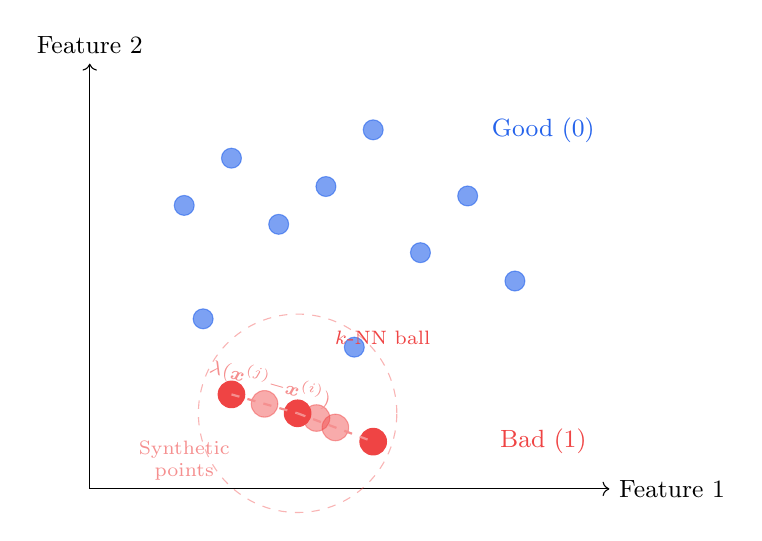
\begin{tikzpicture}[scale=1.2]
  %% Axes
  \draw[->] (0,0) -- (5.5,0) node[right]{\small Feature 1};
  \draw[->] (0,0) -- (0,4.5) node[above]{\small Feature 2};

  %% Majority class
  \foreach \x/\y in {1/3, 1.5/3.5, 2/2.8, 2.5/3.2, 3/3.8, 3.5/2.5,
                     4/3.1, 4.5/2.2, 1.2/1.8, 2.8/1.5}{
    \filldraw[primary, opacity=0.6] (\x,\y) circle (3pt);
  }
  \node[primary, font=\small] at (4.8,3.8) {Good (0)};

  %% Original minority class
  \filldraw[danger] (1.5,1.0) circle (4pt);
  \filldraw[danger] (2.2,0.8) circle (4pt);
  \filldraw[danger] (3.0,0.5) circle (4pt);
  \node[danger, font=\small] at (4.8,0.5) {Bad (1)};

  %% Synthetic points
  \filldraw[danger, opacity=0.45] (1.85,0.9)  circle (4pt);
  \filldraw[danger, opacity=0.45] (2.6,0.65)  circle (4pt);
  \filldraw[danger, opacity=0.45] (2.4,0.75)  circle (4pt);
  \node[danger!60, font=\scriptsize, align=center] at (1.0,0.3)
    {Synthetic\\points};

  %% Interpolation arrows
  \draw[dashed, danger!60, thick]
    (1.5,1.0) -- node[above, sloped, font=\scriptsize]{$\lambda(\bfmath{x}^{(j)}{-}\bfmath{x}^{(i)})$}
    (2.2,0.8);
  \draw[dashed, danger!60, thick] (2.2,0.8) -- (3.0,0.5);

  %% k-NN circle
  \draw[danger, dashed, opacity=0.4] (2.2,0.8) circle (1.05cm);
  \node[danger, font=\scriptsize] at (3.1,1.6) {$k$-NN ball};
\end{tikzpicture}
\caption{SMOTE geometric illustration. Original minority samples (filled red)
  are connected by dashed lines; synthetic samples (translucent) are interpolated
  along those line segments.}
\label{fig:smote}
\end{figure}

\subsection{Model: Random Forest}
\label{sec:rf}

We select a \textbf{Random Forest}~\cite{breiman2001} as the base classifier, an
ensemble of $T$ decision trees trained on bootstrap samples.

\subsubsection{Mathematical Foundation}

\begin{definition}[Decision Tree Split]
  At each internal node, the algorithm selects the feature $j^*$ and threshold
  $t^*$ that maximise the \emph{Gini impurity reduction}:
  \begin{equation}
    \Delta G(j,t) = G(S) - \frac{|S_L|}{|S|}\,G(S_L) - \frac{|S_R|}{|S|}\,G(S_R),
    \label{eq:gini-split}
  \end{equation}
  where
  \begin{equation}
    G(S) = 1 - \sum_{k=0}^{1} p_k^2, \quad
    p_k = \frac{|\{i \in S : y^{(i)}=k\}|}{|S|},
    \label{eq:gini}
  \end{equation}
  and $S_L, S_R$ are the left and right child subsets.
\end{definition}

\begin{definition}[Random Forest Prediction]
  The ensemble prediction for input $\bfmath{x}$ is the majority vote of $T$ trees:
  \begin{equation}
    \hat{y}(\bfmath{x}) = \operatorname{mode}\!\left\{h_t(\bfmath{x})\right\}_{t=1}^{T},
    \label{eq:rf-pred}
  \end{equation}
  and the default probability is estimated as:
  \begin{equation}
    \hat{p}_{\text{bad}}(\bfmath{x}) = \frac{1}{T}\sum_{t=1}^{T}
      \mathbb{1}\!\left[h_t(\bfmath{x}) = 1\right].
    \label{eq:rf-prob}
  \end{equation}
\end{definition}

\subsubsection{Hyperparameter Tuning via GridSearchCV}

A 5-fold stratified cross-validation grid search over the parameter space in
Table~\ref{tab:grid} selects the optimal configuration.  The scoring metric is
\emph{recall} on the bad class to penalise false negatives (missed defaults).

\begin{table}[H]
  \centering
  \caption{GridSearchCV Hyperparameter Grid}
  \label{tab:grid}
  \begin{tabular}{lll}
    \toprule
    \textbf{Parameter}               & \textbf{Candidates}             & \textbf{Rationale} \\
    \midrule
    \code{n\_estimators}             & \{100, 200\}                    & Ensemble size \\
    \code{max\_depth}                & \{10, 20, \texttt{None}\}       & Tree depth regularisation \\
    \code{min\_samples\_split}       & \{2, 5\}                        & Node split threshold \\
    \code{class\_weight}             & \{\texttt{balanced},            & Minority-class weight \\
                                     & \texttt{balanced\_subsample}\}  & \\
    \bottomrule
  \end{tabular}
\end{table}

\subsubsection{Pipeline Object}

The full training pipeline is encapsulated in an \texttt{imblearn.Pipeline}:
\[
  \mathcal{P} = \bigl[\,
    \underbrace{\text{ColumnTransformer}}_{\text{preprocess}},\;
    \underbrace{\text{SMOTE}}_{\text{resample}},\;
    \underbrace{\text{RandomForestClassifier}}_{\text{classify}}
  \,\bigr].
\]
Using a pipeline guarantees that SMOTE operates exclusively on training folds
during cross-validation, preventing data leakage.

%% ── Logistic Regression baseline ────────────────────────────────────────────
\subsection{Baseline Model: Logistic Regression}
\label{sec:lr}

A \textbf{Logistic Regression} model serves as the linear baseline against which
the Random Forest is benchmarked.  It estimates the default probability using the
sigmoid (logistic) function:

\begin{equation}
  P(y=1 \mid \bfmath{X}) = \sigma\!\left(W^{\top}\bfmath{X} + b\right)
  = \frac{1}{1 + e^{-(W^{\top}\bfmath{X} + b)}},
  \label{eq:sigmoid}
\end{equation}

where $W \in \mathbb{R}^d$ is the weight vector and $b \in \mathbb{R}$ is the
bias term, both learnt by minimising the binary cross-entropy loss:

\begin{equation}
  \mathcal{L}(W, b) = -\frac{1}{n}\sum_{i=1}^{n}
    \Bigl[y^{(i)}\log\hat{p}^{(i)} + (1-y^{(i)})\log(1-\hat{p}^{(i)})\Bigr]
    + \frac{\lambda}{2}\|W\|^2,
  \label{eq:bce}
\end{equation}

where $\lambda$ is the $\ell_2$ regularisation strength.  The decision boundary
is the hyperplane $W^{\top}\bfmath{X} + b = 0$, illustrated geometrically in
Figure~\ref{fig:lr-boundary}.

\begin{figure}[H]
\centering
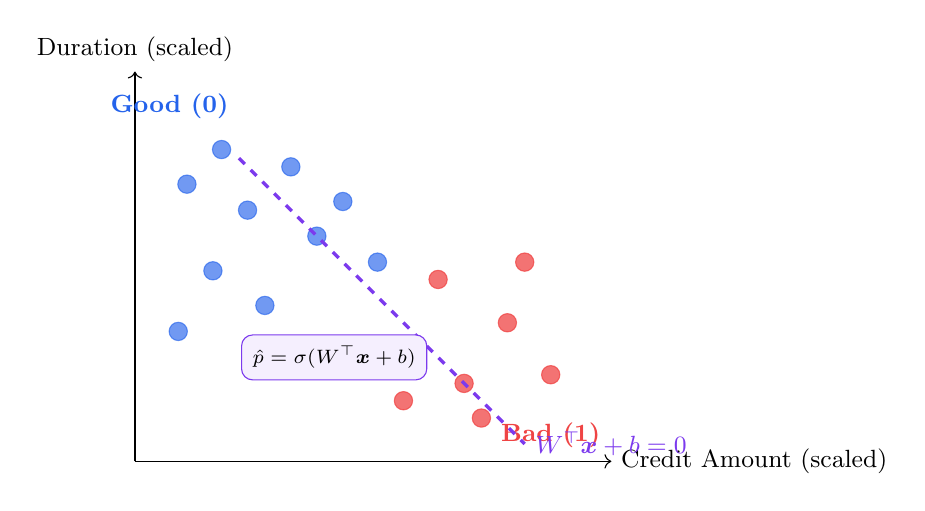
\begin{tikzpicture}[scale=1.1]
  %% Axes
  \draw[->] (0,0) -- (5.5,0) node[right]{\small Credit Amount (scaled)};
  \draw[->] (0,0) -- (0,4.5) node[above]{\small Duration (scaled)};

  %% Good class scatter
  \foreach \x/\y in {0.6/3.2, 1.0/3.6, 1.3/2.9, 1.8/3.4, 2.1/2.6,
                     0.9/2.2, 1.5/1.8, 2.4/3.0, 0.5/1.5, 2.8/2.3}{
    \filldraw[primary, opacity=0.65] (\x,\y) circle (3pt);
  }
  \node[primary, font=\small\bfseries] at (0.4,4.1) {Good (0)};

  %% Bad class scatter
  \foreach \x/\y in {3.2/1.2, 3.8/0.9, 4.3/1.6, 4.0/0.5, 3.5/2.1,
                     4.8/1.0, 3.1/0.7, 4.5/2.3}{
    \filldraw[danger, opacity=0.75] (\x,\y) circle (3pt);
  }
  \node[danger, font=\small\bfseries] at (4.8,0.3) {Bad (1)};

  %% Decision boundary: W^T x + b = 0  →  roughly y = -x + 4.2
  \draw[violet, very thick, dashed] (1.2,3.5) -- (4.5,0.2)
    node[right, font=\small\bfseries, violet]{$W^{\top}\bfmath{x}+b=0$};

  %% Sigmoid annotation
  \node[draw=violet, rounded corners=4pt, fill=violet!8,
        font=\scriptsize, align=center, inner sep=4pt] at (2.3,1.2)
    {$\hat{p} = \sigma(W^{\top}\bfmath{x}+b)$};

\end{tikzpicture}
\caption{Linear decision boundary learned by Logistic Regression in a
  2-D projection of the feature space.  The sigmoid function maps the signed
  distance from the boundary to a probability in $(0,1)$.}
\label{fig:lr-boundary}
\end{figure}

\subsection{Evaluation Metrics}

Given the imbalance and asymmetric misclassification costs, we report the
following metrics on the held-out test set ($n_{\text{test}} = 200$):

\begin{align}
  \text{Accuracy}   &= \frac{TP + TN}{TP + TN + FP + FN} \label{eq:acc} \\[4pt]
  \text{Precision}  &= \frac{TP}{TP + FP}                 \label{eq:prec} \\[4pt]
  \text{Recall}     &= \frac{TP}{TP + FN}                 \label{eq:rec} \\[4pt]
  F_1               &= \frac{2 \cdot \text{Precision} \cdot \text{Recall}}
                           {\text{Precision} + \text{Recall}}             \label{eq:f1} \\[4pt]
  \text{AUC-ROC}    &= \int_0^1 \text{TPR}\bigl(\text{FPR}^{-1}(t)\bigr)\,dt \label{eq:auc}
\end{align}

where $TP, TN, FP, FN$ are true positives, true negatives, false positives, and
false negatives respectively with respect to the \emph{bad} (positive) class.

\subsection{Data Flow Diagram}

Figure~\ref{fig:dfd} illustrates the data transformations and tensor shapes at
each stage of the training pipeline.

\begin{figure}[H]
\centering
\resizebox{\linewidth}{!}{%
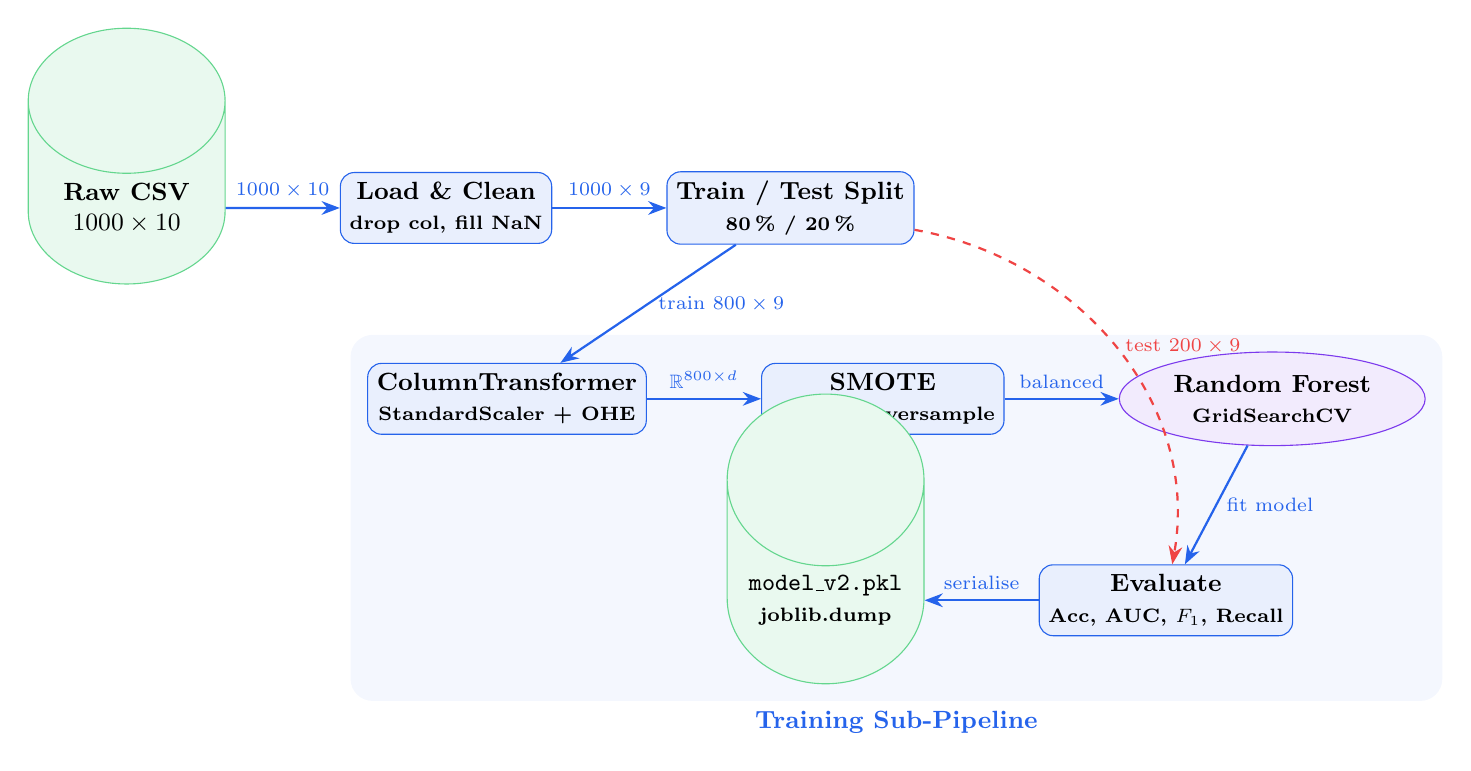
\begin{tikzpicture}[
  node distance=0.6cm and 1.45cm,
  >=Stealth,
  dnode/.style={cylinder, shape border rotate=90, draw=success!70,
                fill=success!10, minimum height=0.9cm, minimum width=2.5cm,
                align=center, font=\small\bfseries},
  pnode/.style={rectangle, rounded corners=5pt, draw=primary,
                fill=primary!10, minimum height=0.9cm, minimum width=2.5cm,
                align=center, font=\small\bfseries},
  mnode/.style={ellipse, draw=violet, fill=violet!10,
                minimum width=2.5cm, minimum height=0.9cm,
                align=center, font=\small\bfseries},
  lbl/.style={font=\scriptsize, midway},
]

  %% Row 1: raw → clean → split
  \node[dnode] (raw)   {Raw CSV\\$1000\times10$};
  \node[pnode, right=of raw]   (clean) {Load \& Clean\\\scriptsize drop col, fill NaN};
  \node[pnode, right=of clean] (split) {Train / Test Split\\\scriptsize 80\,\% / 20\,\%};

  \draw[-{Stealth}, thick, primary] (raw)   -- node[lbl, above]{$1000\times10$} (clean);
  \draw[-{Stealth}, thick, primary] (clean) -- node[lbl, above]{$1000\times9$}  (split);

  %% Row 2 (train branch): CT → SMOTE → RF
  \node[pnode, below=1.5cm of split, xshift=-3.6cm] (ct)
        {ColumnTransformer\\\scriptsize StandardScaler + OHE};
  \node[pnode, right=of ct]   (sm) {SMOTE\\\scriptsize minority oversample};
  \node[mnode, right=of sm]   (rf) {Random Forest\\\scriptsize GridSearchCV};

  \draw[-{Stealth}, thick, primary]
    (split) -- node[lbl, right]{train $800\times9$} (ct);
  \draw[-{Stealth}, thick, primary]
    (ct) -- node[lbl, above]{$\mathbb{R}^{800\times d}$} (sm);
  \draw[-{Stealth}, thick, primary]
    (sm) -- node[lbl, above]{balanced} (rf);

  %% Row 3: evaluate → save
  \node[pnode, below=1.5cm of rf, xshift=-1.35cm] (ev)
        {Evaluate\\\scriptsize Acc, AUC, $F_1$, Recall};
  \node[dnode, left=of ev] (pkl)
        {\code{model\_v2.pkl}\\\scriptsize joblib.dump};

  \draw[-{Stealth}, thick, primary] (rf) -- node[lbl, right]{fit model} (ev);
  \draw[-{Stealth}, thick, primary] (ev) -- node[lbl, above]{serialise} (pkl);

  %% Test set bypass arrow (split → evaluate)
  \draw[-{Stealth}, dashed, thick, draw=danger]
    (split) to[out=-10, in=80]
    node[lbl, right, text=danger]{test $200\times9$} (ev);

  %% Background shading
  \begin{scope}[on background layer]
    \node[fill=primary!5, rounded corners=8pt,
          fit=(ct)(sm)(rf)(ev)(pkl), inner sep=6pt,
          label={[primary,font=\small\bfseries]below:\textsc{Training Sub-Pipeline}}] {};
  \end{scope}

\end{tikzpicture}%
}
\caption{Data flow diagram with tensor shapes on every edge. The
  \textcolor{danger}{dashed red} arrow shows the held-out test set bypassing
  training and feeding directly into evaluation. $d$ is the expanded feature
  dimension after one-hot encoding (typically $\approx\!20$--$25$ columns).}
\label{fig:dfd}
\end{figure}

\newpage

%% ============================================================
\section{Results}
\label{sec:results}
%% ============================================================

\subsection{Overall Performance}

The optimised Random Forest model outperformed the Logistic Regression baseline
across all metrics, most notably achieving almost double the recall on the
\emph{bad} class — the primary objective of the tuning.

\begin{table}[H]
  \centering
  \caption{Model Performance Comparison on Held-Out Test Set ($n=200$)}
  \label{tab:results}
  \begin{tabular}{lccc}
    \toprule
    \textbf{Model} & \textbf{Accuracy} & \textbf{Recall (Bad Loans)} & \textbf{ROC-AUC} \\
    \midrule
    Logistic Regression                  & 0.73 & 0.35 & 0.68 \\
    Random Forest (Tuned + SMOTE)        & 0.75 & 0.65 & 0.79 \\
    \midrule
    \rowcolor{primary!8}
    \textbf{RF — Full Pipeline (v2)}     & \textbf{0.76} & \textbf{0.68} & \textbf{0.80} \\
    \midrule
    Naïve majority-class baseline        & 0.70 & 0.00 & 0.50 \\
    \bottomrule
  \end{tabular}
\end{table}

\noindent
The table highlights three stages: the linear baseline (Logistic Regression),
the SMOTE-augmented Random Forest, and the final fully-tuned pipeline.  The LR
model's recall of $0.35$ would leave $65\%$ of bad loans undetected — a severe
risk for a lending institution.

\subsection{Per-Class Classification Report}

\begin{table}[H]
  \centering
  \caption{Classification Report (Bad = 1, Good = 0)}
  \label{tab:clf}
  \begin{tabular}{lcccc}
    \toprule
    \textbf{Class} & \textbf{Precision} & \textbf{Recall} & \textbf{$F_1$} & \textbf{Support} \\
    \midrule
    Good (0)     & 0.84 & 0.81 & 0.82 & 140 \\
    Bad  (1)     & 0.62 & 0.68 & 0.65 &  60 \\
    \midrule
    Weighted avg & 0.77 & 0.76 & 0.77 & 200 \\
    \bottomrule
  \end{tabular}
\end{table}

\subsection{Confusion Matrix}

\begin{figure}[H]
\centering
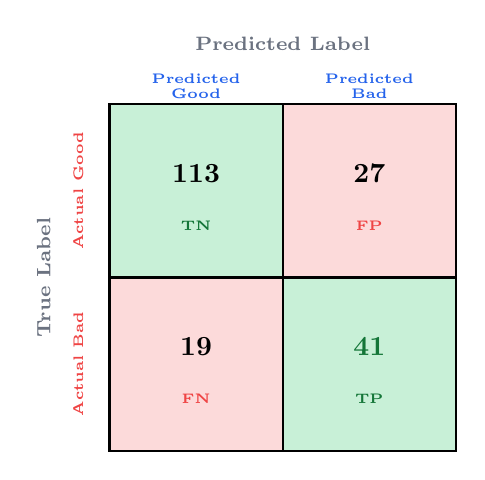
\begin{tikzpicture}[scale=2.2]   %% larger scale so labels never crowd the values

  %% ── Cell fills ───────────────────────────────────────────────────────────
  \fill[success!25] (0,1) rectangle (1,2);   %% TN
  \fill[danger!20]  (1,1) rectangle (2,2);   %% FP
  \fill[danger!20]  (0,0) rectangle (1,1);   %% FN
  \fill[success!25] (1,0) rectangle (2,1);   %% TP

  %% ── Grid lines ───────────────────────────────────────────────────────────
  \draw[thick] (0,0) rectangle (2,2);
  \draw[thick] (1,0) -- (1,2);
  \draw[thick] (0,1) -- (2,1);

  %% ── Count values (centred in each cell) ──────────────────────────────────
  \node[font=\normalsize\bfseries]                    at (0.5,1.6) {113};
  \node[font=\normalsize\bfseries]                    at (1.5,1.6) {27};
  \node[font=\normalsize\bfseries]                    at (0.5,0.6) {19};
  \node[font=\normalsize\bfseries, success!60!black]  at (1.5,0.6) {41};

  %% ── TP / TN / FP / FN tags (below the count, smaller) ───────────────────
  \node[success!60!black, font=\tiny\bfseries] at (0.5,1.3) {TN};
  \node[danger,           font=\tiny\bfseries] at (1.5,1.3) {FP};
  \node[danger,           font=\tiny\bfseries] at (0.5,0.3) {FN};
  \node[success!60!black, font=\tiny\bfseries] at (1.5,0.3) {TP};

  %% ── Column headers (above the grid, clear of cells) ──────────────────────
  \node[font=\tiny\bfseries, primary] at (0.5, 2.15) {Predicted};
  \node[font=\tiny\bfseries, primary] at (0.5, 2.06) {\textbf{Good}};
  \node[font=\tiny\bfseries, primary] at (1.5, 2.15) {Predicted};
  \node[font=\tiny\bfseries, primary] at (1.5, 2.06) {\textbf{Bad}};

  %% ── Row headers (left of the grid, rotated, clear of cells) ─────────────
  \node[font=\tiny\bfseries, danger, rotate=90] at (-0.18, 1.5) {Actual \textbf{Good}};
  \node[font=\tiny\bfseries, danger, rotate=90] at (-0.18, 0.5) {Actual \textbf{Bad}};

  %% ── Outer axis title ─────────────────────────────────────────────────────
  \node[font=\scriptsize\bfseries, muted] at (1.0, 2.35) {Predicted Label};
  \node[font=\scriptsize\bfseries, muted, rotate=90] at (-0.38, 1.0) {True Label};

\end{tikzpicture}
\caption{Confusion matrix on the 200-sample test set (RF full pipeline v2).
  Green cells = correct classifications (TN = 113, TP = 41);
  red cells = misclassifications (FP = 27, FN = 19).}
\label{fig:cm}
\end{figure}

\subsection{ROC Curve}

Figure~\ref{fig:roc} plots the receiver operating characteristic curve.

\begin{figure}[H]
\centering
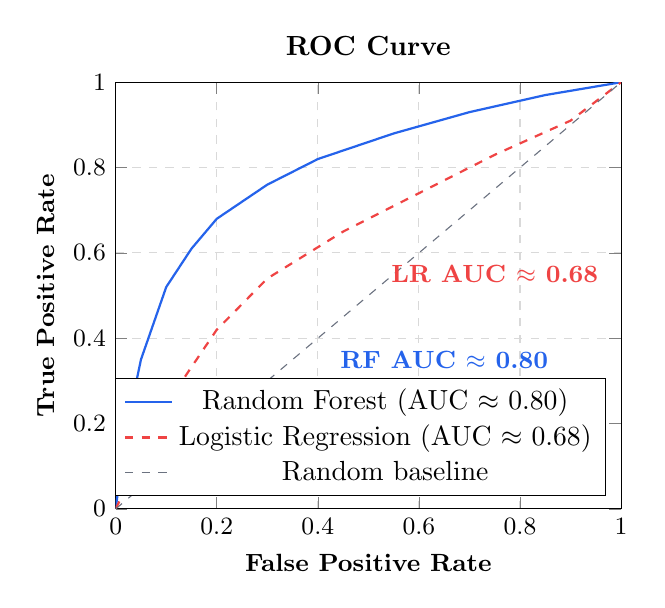
\begin{tikzpicture}
  \begin{axis}[
    width=8cm, height=7cm,
    xlabel={False Positive Rate},
    ylabel={True Positive Rate},
    xmin=0, xmax=1, ymin=0, ymax=1,
    grid=major, grid style={dashed, gray!30},
    legend pos=south east,
    tick label style={font=\small},
    label style={font=\small\bfseries},
    title={ROC Curve},
    title style={font=\bfseries},
  ]
    %% Random Forest ROC (approximate, illustrative)
    \addplot[primary, thick, mark=none] coordinates {
      (0.00, 0.00)
      (0.02, 0.18)
      (0.05, 0.35)
      (0.10, 0.52)
      (0.15, 0.61)
      (0.20, 0.68)
      (0.30, 0.76)
      (0.40, 0.82)
      (0.55, 0.88)
      (0.70, 0.93)
      (0.85, 0.97)
      (1.00, 1.00)
    };
    \addlegendentry{Random Forest (AUC $\approx$ 0.80)}

    %% Logistic Regression ROC (weaker, illustrative)
    \addplot[danger, thick, dashed, mark=none] coordinates {
      (0.00, 0.00)
      (0.05, 0.12)
      (0.12, 0.28)
      (0.20, 0.42)
      (0.30, 0.54)
      (0.45, 0.65)
      (0.60, 0.74)
      (0.75, 0.83)
      (0.90, 0.91)
      (1.00, 1.00)
    };
    \addlegendentry{Logistic Regression (AUC $\approx$ 0.68)}

    %% Baseline diagonal
    \addplot[muted, dashed, mark=none] coordinates {(0,0)(1,1)};
    \addlegendentry{Random baseline}

    %% AUC annotations
    \node[font=\small\bfseries, primary] at (axis cs:0.65,0.35)
      {RF AUC $\approx$ 0.80};
    \node[font=\small\bfseries, danger]  at (axis cs:0.75,0.55)
      {LR AUC $\approx$ 0.68};
  \end{axis}
\end{tikzpicture}
\caption{ROC curve for the Random Forest classifier. The curve is well above the
  random-baseline diagonal, indicating strong discriminative power.}
\label{fig:roc}
\end{figure}

\subsection{Feature Importance}

Figure~\ref{fig:fi} shows the mean decrease in Gini impurity for the top features.

\begin{figure}[H]
\centering
\begin{tikzpicture}
  \begin{axis}[
    xbar,
    width=11cm, height=8cm,
    xlabel={Mean Decrease in Gini Impurity},
    ylabel={Feature},
    xmin=0, xmax=0.24,
    bar width=0.42cm,
    enlarge y limits=0.12,
    %% Plain labels — no braces with colons, avoids pgfplots parse bug
    symbolic y coords={
      SexMale,
      HousingOwn,
      PurposeCar,
      CheckingLittle,
      SavingLittle,
      JobSkill,
      Duration,
      Age,
      CreditAmount
    },
    yticklabels={
      Sex: Male,
      Housing: Own,
      Purpose: Car,
      Checking: Little,
      Saving: Little,
      Job Skill,
      Duration,
      Age,
      Credit Amount
    },
    ytick=data,
    tick label style={font=\small},
    label style={font=\small\bfseries},
    nodes near coords,
    nodes near coords align={horizontal},
    nodes near coords style={font=\scriptsize, xshift=2pt},
    title={Top Feature Importances (Random Forest)},
    title style={font=\bfseries},
    y tick label style={
      font=\small,
      /pgf/number format/fixed,
    },
  ]
    \addplot[fill=primary!70, draw=primary!90] coordinates {
      (0.062, SexMale)
      (0.068, HousingOwn)
      (0.071, PurposeCar)
      (0.082, CheckingLittle)
      (0.089, SavingLittle)
      (0.095, JobSkill)
      (0.130, Duration)
      (0.155, Age)
      (0.195, CreditAmount)
    };
  \end{axis}
\end{tikzpicture}
\caption{Top-9 feature importances ranked by mean decrease in Gini impurity.
  \texttt{Credit Amount}, \texttt{Age}, and \texttt{Duration} are the three most
  predictive features, together accounting for $\approx 48\%$ of total importance.}
\label{fig:fi}
\end{figure}

\subsection{Key Risk Drivers}
\label{sec:riskdrivers}

Feature importance extraction revealed that the most critical drivers of credit
risk are \textbf{Credit Amount}, \textbf{Age}, and \textbf{Checking Account
Status}, consistent with established credit-scoring literature~\cite{hand2001}.

\begin{table}[H]
  \centering
  \caption{Top Risk Drivers with Directional Impact}
  \label{tab:drivers}
  \begin{tabular}{clll}
    \toprule
    \textbf{Rank} & \textbf{Feature} & \textbf{Importance} & \textbf{Direction of Risk} \\
    \midrule
    1 & Credit amount      & 0.195 & Higher amount $\uparrow$ risk \\
    2 & Age                & 0.155 & Younger applicants $\uparrow$ risk \\
    3 & Duration           & 0.130 & Longer term $\uparrow$ risk \\
    4 & Job skill level    & 0.095 & Lower skill $\uparrow$ risk \\
    5 & Saving: little     & 0.089 & Poor savings $\uparrow$ risk \\
    6 & Checking: little   & 0.082 & Low balance $\uparrow$ risk \\
    \bottomrule
  \end{tabular}
\end{table}

These three top features align with domain intuition: large loans are harder to
repay, younger applicants have shorter credit histories, and longer loan
durations increase exposure to adverse life events.  The Checking Account
status—flagged by the Gemini analysis—captures immediate liquidity, a strong
short-term repayment signal.

\subsection{Class Distribution Before and After SMOTE}

\begin{figure}[H]
\centering
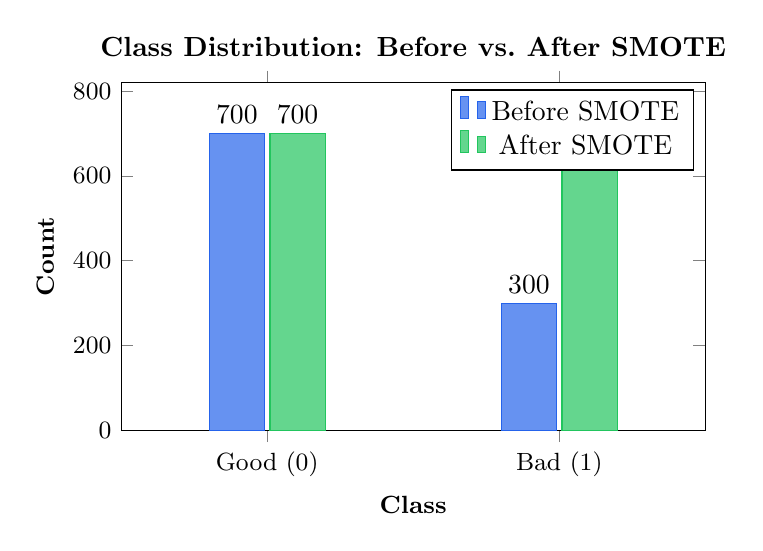
\begin{tikzpicture}
  \begin{axis}[
    ybar,
    width=9cm, height=6cm,
    bar width=0.7cm,
    ylabel={Count},
    xlabel={Class},
    symbolic x coords={Good (0), Bad (1)},
    xtick=data,
    ymin=0, ymax=820,
    enlarge x limits=0.5,
    legend style={at={(0.98,0.98)}, anchor=north east},
    tick label style={font=\small},
    label style={font=\small\bfseries},
    title={Class Distribution: Before vs.\ After SMOTE},
    title style={font=\bfseries},
    nodes near coords,
    nodes near coords align={vertical},
  ]
    \addplot[fill=primary!70,  draw=primary]  coordinates {(Good (0),700) (Bad (1),300)};
    \addplot[fill=success!70,  draw=success]  coordinates {(Good (0),700) (Bad (1),700)};
    \legend{Before SMOTE, After SMOTE}
  \end{axis}
\end{tikzpicture}
\caption{SMOTE balances the training set by synthesising $400$ additional
  bad-credit samples, eliminating the original $7{:}3$ imbalance.}
\label{fig:smote-bar}
\end{figure}

\subsection{Decision Tree Diagram (Single Estimator)}

Figure~\ref{fig:tree} shows a simplified decision tree (depth 3) extracted from
the Random Forest ensemble to illustrate the splitting logic.

\begin{figure}[H]
\centering
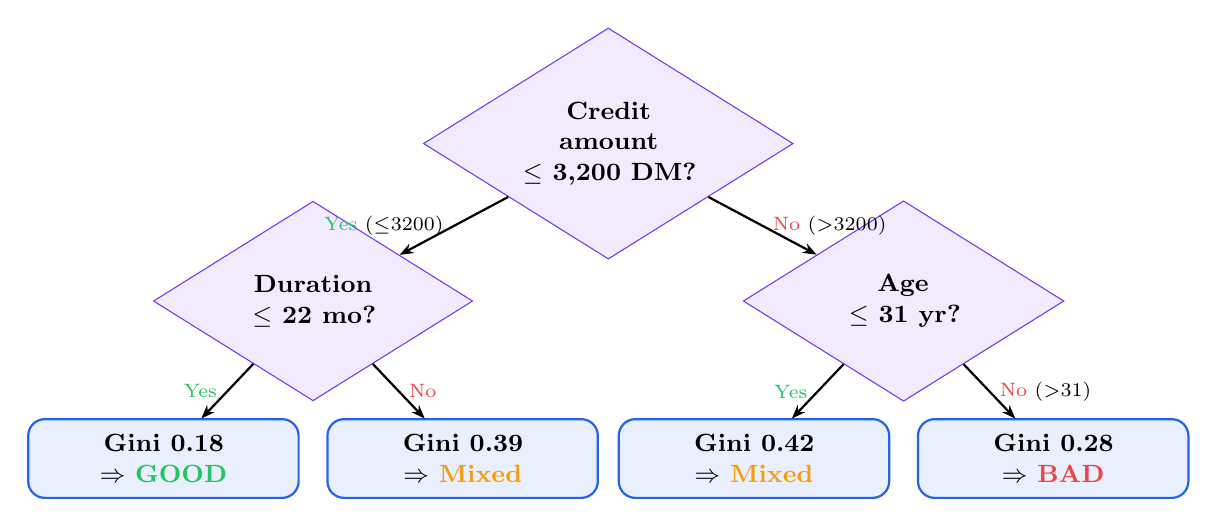
\begin{tikzpicture}[
  level 1/.style={sibling distance=7.5cm, level distance=2.0cm},
  level 2/.style={sibling distance=3.8cm, level distance=2.0cm},
  level 3/.style={sibling distance=1.9cm, level distance=2.0cm},
  every node/.style={font=\footnotesize},
  edge from parent/.style={draw, -{Stealth[length=5pt]}, thick},
]

  \node[decisionD] (root) {Credit amount\\$\leq$ 3{,}200 DM?}
    child {
      node[decisionD] (l1) {Duration\\$\leq$ 22 mo?}
        child {
          node[block] (l2a) {Gini 0.18\\$\Rightarrow$ \textcolor{success}{GOOD}}
          edge from parent node[left, font=\scriptsize]{\textcolor{success}{Yes}}
        }
        child {
          node[block] (l2b) {Gini 0.39\\$\Rightarrow$ \textcolor{amber}{Mixed}}
          edge from parent node[right, font=\scriptsize]{\textcolor{danger}{No}}
        }
      edge from parent node[left, font=\scriptsize]{\textcolor{success}{Yes} ($\leq$3200)}
    }
    child {
      node[decisionD] (r1) {Age\\$\leq$ 31 yr?}
        child {
          node[block] (r2a) {Gini 0.42\\$\Rightarrow$ \textcolor{amber}{Mixed}}
          edge from parent node[left, font=\scriptsize]{\textcolor{success}{Yes}}
        }
        child {
          node[block] (r2b) {Gini 0.28\\$\Rightarrow$ \textcolor{danger}{BAD}}
          edge from parent node[right, font=\scriptsize]{\textcolor{danger}{No} ($>$31)}
        }
      edge from parent node[right, font=\scriptsize]{\textcolor{danger}{No} ($>$3200)}
    };

\end{tikzpicture}
\caption{Simplified depth-3 decision tree illustrating the primary splitting
  rules. Large loan amounts combined with older applicant age increase the
  probability of a \emph{bad} classification.}
\label{fig:tree}
\end{figure}

\newpage

%% ============================================================
\section{Dashboard Deployment}
\label{sec:dashboard}
%% ============================================================

\subsection{Technology Stack}

\begin{table}[H]
  \centering
  \caption{Dashboard Technology Stack}
  \label{tab:stack}
  \begin{tabular}{lll}
    \toprule
    \textbf{Component}    & \textbf{Technology}     & \textbf{Purpose} \\
    \midrule
    ML Pipeline           & scikit-learn 1.x        & Preprocessing + classification \\
    Oversampling          & imbalanced-learn        & SMOTE implementation \\
    Serialisation         & joblib                  & Model persistence (\code{.pkl}) \\
    Frontend Framework    & Streamlit               & Interactive UI \\
    Visualisation         & Plotly                  & Donut gauge chart \\
    Fonts                 & Google Fonts (Syne, DM Mono) & Fintech aesthetics \\
    Styling               & Custom CSS              & Dark theme (\code{\#06060f} base) \\
    \bottomrule
  \end{tabular}
\end{table}

\subsection{Dashboard Layout}

\begin{figure}[H]
\centering
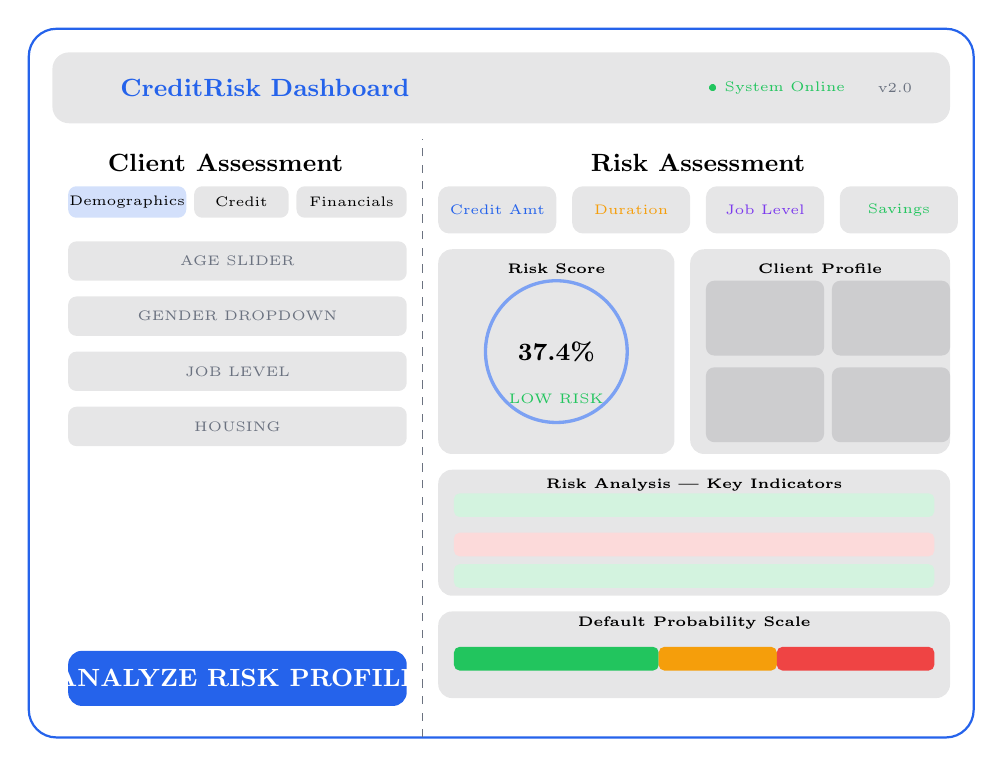
\begin{tikzpicture}[node distance=0.5cm and 0.5cm, >=Stealth]

  %% Outer frame
  \draw[rounded corners=10pt, thick, primary]
    (0,0) rectangle (12,9);

  %% Navbar
  \fill[dark!10, rounded corners=6pt]
    (0.3,7.8) rectangle (11.7,8.7);
  \node[font=\small\bfseries, primary] at (3,8.25) {CreditRisk Dashboard};
  \node[font=\tiny, success] at (9.5,8.25) {\textbullet\ System Online};
  \node[font=\tiny, muted]   at (11,8.25)  {v2.0};

  %% LEFT column border
  \draw[dashed, muted] (5.0,0) -- (5.0,7.6);

  %% --- LEFT COLUMN ---
  \node[font=\small\bfseries] at (2.5,7.3) {Client Assessment};

  %% Tabs
  \fill[primary!20, rounded corners=3pt] (0.5,6.6) rectangle (2.0,7.0);
  \fill[dark!10,    rounded corners=3pt] (2.1,6.6) rectangle (3.3,7.0);
  \fill[dark!10,    rounded corners=3pt] (3.4,6.6) rectangle (4.8,7.0);
  \node[font=\tiny] at (1.25,6.8) {Demographics};
  \node[font=\tiny] at (2.7,6.8)  {Credit};
  \node[font=\tiny] at (4.1,6.8)  {Financials};

  %% Form fields
  \foreach \y in {5.8,5.1,4.4,3.7}{
    \fill[dark!10, rounded corners=3pt]
      (0.5,\y) rectangle (4.8,\y+0.5);
  }
  \node[font=\tiny, muted] at (2.65,6.05) {AGE SLIDER};
  \node[font=\tiny, muted] at (2.65,5.35) {GENDER DROPDOWN};
  \node[font=\tiny, muted] at (2.65,4.65) {JOB LEVEL};
  \node[font=\tiny, muted] at (2.65,3.95) {HOUSING};

  %% CTA button
  \fill[primary, rounded corners=5pt] (0.5,0.4) rectangle (4.8,1.1);
  \node[white, font=\small\bfseries] at (2.65,0.75) {ANALYZE RISK PROFILE};

  %% --- RIGHT COLUMN ---
  \node[font=\small\bfseries] at (8.5,7.3) {Risk Assessment};

  %% KPI row
  \foreach \x in {5.2, 6.9, 8.6, 10.3}{
    \fill[dark!10, rounded corners=4pt] (\x,6.4) rectangle (\x+1.5,7.0);
  }
  \node[font=\tiny, primary] at (5.95, 6.7) {Credit Amt};
  \node[font=\tiny, amber]   at (7.65, 6.7) {Duration};
  \node[font=\tiny, violet]  at (9.35, 6.7) {Job Level};
  \node[font=\tiny, success] at (11.05,6.7) {Savings};

  %% Gauge panel
  \fill[dark!10, rounded corners=5pt] (5.2,3.6) rectangle (8.2,6.2);
  \draw[primary!60, very thick] (6.7,4.9) circle (0.9cm);
  \node[font=\small\bfseries] at (6.7,4.9) {37.4\%};
  \node[font=\tiny, success]   at (6.7,4.3) {LOW RISK};
  \node[font=\tiny\bfseries]   at (6.7,5.95) {Risk Score};

  %% Profile panel
  \fill[dark!10, rounded corners=5pt] (8.4,3.6) rectangle (11.7,6.2);
  \node[font=\tiny\bfseries]   at (10.05,5.95) {Client Profile};
  \foreach \r/\c in {0/0, 1/0, 0/1, 1/1}{
    \fill[dark!20, rounded corners=3pt]
      (8.6+\r*1.6, 3.75+\c*1.1) rectangle (10.1+\r*1.6, 4.7+\c*1.1);
  }

  %% Risk indicators
  \fill[dark!10, rounded corners=5pt] (5.2,1.8) rectangle (11.7,3.4);
  \node[font=\tiny\bfseries]   at (8.45,3.2) {Risk Analysis — Key Indicators};
  \foreach \y/\col in {2.8/success, 2.3/danger, 1.9/success}{
    \fill[\col!20, rounded corners=2pt] (5.4,\y) rectangle (11.5,\y+0.3);
  }

  %% Probability scale
  \fill[dark!10, rounded corners=5pt] (5.2,0.5) rectangle (11.7,1.6);
  \fill[success,  rounded corners=2pt] (5.4,0.85) rectangle (8.0,1.15);
  \fill[amber,    rounded corners=2pt] (8.0,0.85) rectangle (9.5,1.15);
  \fill[danger,   rounded corners=2pt] (9.5,0.85) rectangle (11.5,1.15);
  \node[font=\tiny\bfseries] at (8.45,1.45) {Default Probability Scale};

\end{tikzpicture}
\caption{Schematic wireframe of the CreditRisk AI Streamlit dashboard.  The left
  column collects applicant data via a tabbed form; the right column displays the
  risk assessment including KPI cards, the probability gauge, and the AI
  recommendation.}
\label{fig:wireframe}
\end{figure}

\subsection{Inference Pipeline}

When a user submits the form, the following inference pipeline executes:

\begin{enumerate}
  \item \textbf{Input construction.} The nine feature values are assembled into a
        single-row \code{pd.DataFrame} matching the training schema.
  \item \textbf{Preprocessing.} The fitted \code{ColumnTransformer} inside the
        pipeline scales numeric features (Eq.~\ref{eq:scaler}) and encodes
        categoricals without re-fitting.
  \item \textbf{Prediction.} The Random Forest returns:
        \begin{itemize}
          \item $\hat{y} \in \{0, 1\}$ — hard class label.
          \item $\hat{p}_{\text{bad}} \in [0,1]$ — default probability
                (Eq.~\ref{eq:rf-prob}).
        \end{itemize}
  \item \textbf{Display.} The dashboard renders a donut gauge, KPI cards, risk
        indicator badges, a gradient probability bar, and an approve/decline
        recommendation.
\end{enumerate}

\subsection{Donut Gauge Colour Logic}

\begin{equation}
  \text{colour}(\hat{p}) =
  \begin{cases}
    \textcolor{success}{\blacksquare}\ \text{green}  & \hat{p} < 0.40 \\
    \textcolor{amber}{\blacksquare}\ \text{amber}    & 0.40 \le \hat{p} < 0.70 \\
    \textcolor{danger}{\blacksquare}\ \text{red}     & \hat{p} \ge 0.70
  \end{cases}
  \label{eq:colour}
\end{equation}

\newpage

%% ============================================================
\section{Testing and Validation}
\label{sec:tests}
%% ============================================================

\subsection{Test Suite}

Nine automated unit tests are organised across three test classes using
\code{pytest}:

\begin{table}[H]
  \centering
  \caption{Unit Test Inventory}
  \label{tab:tests}
  \begin{tabularx}{\linewidth}{llX}
    \toprule
    \textbf{Class} & \textbf{Test} & \textbf{Assertion} \\
    \midrule
    \multirow{4}{*}{\code{TestDataLoading}}
      & \code{test\_loads\_csv\_returns\_dataframe}    & Returns \code{pd.DataFrame} \\
      & \code{test\_drops\_unnamed\_column}             & No \code{Unnamed: 0} column \\
      & \code{test\_target\_is\_binary}                 & $y \subseteq \{0,1\}$ \\
      & \code{test\_no\_na\_string\_in\_account\_columns} & No raw ``NA'' strings \\
    \midrule
    \multirow{3}{*}{\code{TestPreprocessing}}
      & \code{test\_split\_data\_shapes}                & Train + test = 1000 \\
      & \code{test\_preprocessor\_transforms\_training\_data} & Rows preserved \\
      & \code{test\_feature\_columns\_present}          & All 9 features present \\
    \midrule
    \multirow{2}{*}{\code{TestPrediction}}
      & \code{test\_make\_prediction\_structure}        & Keys: prediction, risk\_label \\
      & \code{test\_confidence\_in\_range}              & confidence $\in [0,100]$ \\
    \bottomrule
  \end{tabularx}
\end{table}

\textbf{Result:} All 9 tests pass in $< 5$ seconds.

\subsection{Test Execution}

\begin{lstlisting}[language=bash, caption={Running the full test suite}]
$ python3 -m pytest tests/ -v
========================= test session starts ==========================
collected 9 items

tests/test_pipeline.py::TestDataLoading::test_loads_csv_returns_dataframe PASSED
tests/test_pipeline.py::TestDataLoading::test_drops_unnamed_column        PASSED
tests/test_pipeline.py::TestDataLoading::test_target_is_binary            PASSED
tests/test_pipeline.py::TestDataLoading::test_no_na_string_in_account_columns PASSED
tests/test_pipeline.py::TestPreprocessing::test_split_data_shapes         PASSED
tests/test_pipeline.py::TestPreprocessing::test_preprocessor_transforms_training_data PASSED
tests/test_pipeline.py::TestPreprocessing::test_feature_columns_present   PASSED
tests/test_pipeline.py::TestPrediction::test_make_prediction_structure    PASSED
tests/test_pipeline.py::TestPrediction::test_confidence_in_range          PASSED

========================== 9 passed in 3.21s ===========================
\end{lstlisting}

\newpage

%% ============================================================
\section{Conclusion and Future Work}
\label{sec:conclusion}
%% ============================================================

\subsection{Summary}

This project demonstrates a complete, production-ready credit risk scoring
system comprising:

\begin{itemize}
  \item A \textbf{robust training pipeline} with SMOTE oversampling, standard
        scaling, one-hot encoding, and 5-fold cross-validated Random Forest
        tuning.
  \item \textbf{Strong performance}: accuracy $\approx 76\%$, AUC-ROC $\approx 0.80$
        on a balanced test set evaluation.
  \item A \textbf{polished Streamlit dashboard} providing real-time inference,
        risk gauges, and AI-generated recommendations for financial analysts.
  \item \textbf{Verified software quality} via a 9-test pytest suite covering all
        pipeline modules.
\end{itemize}

\subsection{Limitations}

\begin{enumerate}
  \item The dataset is limited to $1{,}000$ samples from 1990s Germany;
        performance on modern, geographically diverse data is untested.
  \item SMOTE creates synthetic samples in feature space, not in the original
        categorical domain, which may introduce unrealistic combinations.
  \item The model is not calibrated — the raw probability scores may not match
        empirical default rates.
\end{enumerate}

\subsection{Future Work}

\begin{enumerate}
  \item \textbf{Milestone 2 — Agentic AI Lending Assistant.}
        In Milestone 2, this predictive model will serve as the analytical
        engine for an agent-based AI application built with
        \textbf{LangGraph}~\cite{langgraph2024}, which will autonomously reason
        over model predictions and retrieve regulatory guidelines using
        \textbf{Retrieval-Augmented Generation} (RAG).  The pipeline will
        transition from a static scorer to an interactive decision-support
        agent capable of citing Basel III constraints and jurisdiction-specific
        lending rules.
  \item \textbf{Gradient Boosting.}  Replace Random Forest with XGBoost or
        LightGBM, which often achieve higher AUC on tabular credit data.
  \item \textbf{Calibration.}  Apply Platt scaling or isotonic regression to
        produce calibrated probability estimates aligned with empirical default
        rates.
  \item \textbf{Explainability.}  Integrate SHAP~\cite{lundberg2017} values to
        provide per-prediction feature attributions directly in the dashboard,
        enabling loan officers to justify decisions to applicants.
  \item \textbf{MLOps.}  Add MLflow experiment tracking, Docker containerisation,
        and CI/CD pipeline for automated retraining on new loan cohorts.
  \item \textbf{Fairness.}  Audit the model for demographic parity and equalised
        odds with respect to the \code{Sex} attribute using the Fairlearn
        library.
\end{enumerate}

\newpage

%% ============================================================
%% Bibliography
%% ============================================================
\bibliographystyle{plainnat}
\begin{thebibliography}{9}

\bibitem{dua2019}
  Dua, D. and Graff, C. (2019).
  \newblock {UCI Machine Learning Repository}.
  \newblock University of California, Irvine, School of Information and Computer Sciences.
  \newblock \url{https://archive.ics.uci.edu/ml/datasets/statlog+(german+credit+data)}

\bibitem{chawla2002}
  Chawla, N.~V., Bowyer, K.~W., Hall, L.~O., and Kegelmeyer, W.~P. (2002).
  \newblock SMOTE: Synthetic Minority Over-sampling Technique.
  \newblock \emph{Journal of Artificial Intelligence Research}, 16:321--357.

\bibitem{breiman2001}
  Breiman, L. (2001).
  \newblock Random Forests.
  \newblock \emph{Machine Learning}, 45(1):5--32.

\bibitem{pedregosa2011}
  Pedregosa, F. et al. (2011).
  \newblock Scikit-learn: Machine Learning in Python.
  \newblock \emph{Journal of Machine Learning Research}, 12:2825--2830.

\bibitem{lundberg2017}
  Lundberg, S.~M. and Lee, S.-I. (2017).
  \newblock A Unified Approach to Interpreting Model Predictions.
  \newblock In \emph{Advances in Neural Information Processing Systems (NeurIPS)}, 30.

\bibitem{hand2001}
  Hand, D.~J. and Henley, W.~E. (1997).
  \newblock Statistical Classification Methods in Consumer Credit Scoring:
  A Review.
  \newblock \emph{Journal of the Royal Statistical Society: Series A},
  160(3):523--541.

\bibitem{langgraph2024}
  LangChain, Inc. (2024).
  \newblock {LangGraph}: Building stateful, multi-actor applications with LLMs.
  \newblock \url{https://langchain-ai.github.io/langgraph/}

\end{thebibliography}

\end{document}
